\documentclass{standalone}

\usepackage{tikz}
\usetikzlibrary{arrows,calc,shapes,positioning,arrows.meta}


\begin{document}
	\begin{tikzpicture}
		\node at (0,0) {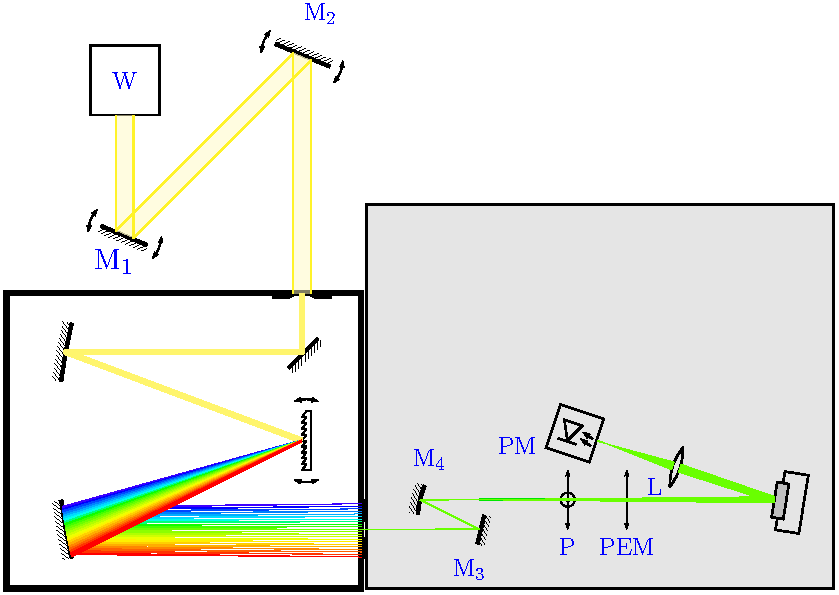
\includegraphics{build/ras-setup}};
		
		
	%	\node at (6.6,-3) {.};
		
		%\draw (6.6,-3)--(6.6,-4.8);

		\draw[blue,line width=1pt]  (6.32,-4.5) -- ++(80+0:1.5) -- +(90:-1.5);
		\draw[red,line width=1pt]  (6.32,-4.5) arc (90:80:1.5);
		
		\node at (6.5,-4.7) {$\approx 4.5^{\circ}$};
		
		\draw[dashed,red](5.9,-3.4) -- (4,-1.1); 
			\draw[dashed,red](6,-3.4) -- (6.5,0); 
	%	\draw(4.6,-3) -- ++(3+4:3) -- +(4:2);
	
\draw[red, semitransparent,fill=white] (5,0) circle[radius=1.5cm];% test of the radius size

\draw[draw=black,fill=white]  (4.1,-1) rectangle ++(1.75,2);
\draw[-Stealth,rotate around={45:(5,-0.5)},blue] (5,-0.5)--(5,0.5);
\draw[-Stealth,rotate around={-45:(5,-0.5)},blue] (5,-0.5)--(5,0.5);
\node[rotate =-45] at (4.5,-0.5) {$\left[1\overline{1}0\right]$};
\node[rotate =45] at (5.5,-0.5) {$\left[110\right]$};
	\end{tikzpicture}
\end{document}